\documentclass{article}


\usepackage{neurips_data_2024}


\usepackage[utf8]{inputenc} % allow utf-8 input
\usepackage[T1]{fontenc}    % use 8-bit T1 fonts
\usepackage{hyperref}       % hyperlinks
\usepackage{url}            % simple URL typesetting
\usepackage{booktabs}       % professional-quality tables
\usepackage{amsfonts}       % blackboard math symbols
\usepackage{nicefrac}       % compact symbols for 1/2, etc.
\usepackage{microtype}      % microtypography
\usepackage{xcolor}         % colors
\usepackage{graphicx} 

\title{Assignment 2: NBA Dataset}


\author{%
 Sean Mahlanza (2438634) \\ 
 Phemelo Masilo (2444482) \\
 Gael Joao (2494554) \\
 Blessing Kodze (2560370) \\
}

\begin{document}

\maketitle

\begin{abstract}
  The abstract paragraph should be indented \nicefrac{1}{2}~inch (3~picas) on
  both the left- and right-hand margins. Use 10~point type, with a vertical
  spacing (leading) of 11~points.  The word \textbf{Abstract} must be centered,
  bold, and in point size 12. Two line spaces precede the abstract. The abstract
  must be limited to one paragraph.
\end{abstract}

\section{Data Cleaning}

The NBA 2022-23 statistics dataset underwent systematic data cleaning and preprocessing to ensure data quality and prepare it for machine learning analysis. First, we removed the redundant index column (\texttt{Unnamed: 0}) that duplicated the DataFrame's built-in index. We then addressed data type inconsistencies, particularly in the \texttt{3P} (3-Point Field Goals Made) column, which contained string values with spurious 's' characters (e.g., '1.s6' instead of '1.6'). Missing values in shooting percentage columns (\texttt{3P\%}, \texttt{FT\%}, \texttt{FG\%}, etc.) were filled with zero, as these typically indicated zero attempts rather than missing data. To address data quality concerns related to players with minimal playing time, we applied minimal filtering criteria, retaining only players with at least 5 games played and 25 total minutes, which removed approximately 467 players with negligible statistical impact while preserving meaningful data. For machine learning applications, we removed identifier columns (\texttt{Player Name}, \texttt{Team}, \texttt{Position}), applied log transformation to the \texttt{Salary} feature to reduce skewness, split the data into training (70\%), validation (15\%), and test (15\%) sets with a fixed random seed (42) for reproducibility, and standardized all features to zero mean and unit variance using \texttt{StandardScaler}. This comprehensive preprocessing pipeline resulted in 48 numeric features ready for dimensionality reduction and clustering analysis.

\section{Dimensionality Reduction}

\subsection{Autoencoders + Self-organising maps}

\begin{table}[h!]
\centering
\caption{Cluster Statistical Summary (mean values per player group)}
\label{tab:cluster_stats}
\begin{tabular}{lcccccc}
\toprule
\textbf{Cluster} & \textbf{PTS} & \textbf{AST\%} & \textbf{STL\%} & \textbf{BLK\%} & \textbf{ORB\%} & \textbf{DRB\%} \\
\midrule
Blue: Rotational contributors & 8.03 & 13.04 & 1.58 & 1.39 & 3.88 &	12.68 \\
Orange: Defensive players & 6.22 & 10.34 & 1.42 & 2.49 & 7.32 & 16.35 \\
Green: Franchise players & 20.58 & 18.58 & 1.36 & 2.74 & 7.92 & 21.35 \\
Red: Deep Bench & 4.81	& 9.89 &	1.43 &	1.90 &	6.54 &	15.55 \\
Purple: Primary Perimeter Scoring Options & 17.42	&20.77 &	1.43 &	1.39	& 3.60	& 14.81 \\
\bottomrule
\end{tabular}
\end{table}

In this section we made use of the latent vectors derived from the autoencoders in 2.1.a combined with a SOMs approach.
The SOMs approach helps us understand the continuous similarity patterns between the player roles, and we later use it to then derive two graphs: U-matrix and the Player cluster. The U-matrix will be used to show class boundaries:

The {\bf light areas} indicate large distances between the neurons which translates to a strong difference between the group of players.
The {\bf dark areas} indicate small distances between the neurons which are homogeneous regions where players have similar profiles.

Finally we use the Player cluster to help us interpretate the different data points in the clusters and their mapping from the U-matrix gradients. Using SOMs and the averages from the statistical summary table, we see that the player roles are more general and not position specific.

\begin{figure}[h]
    \centering
    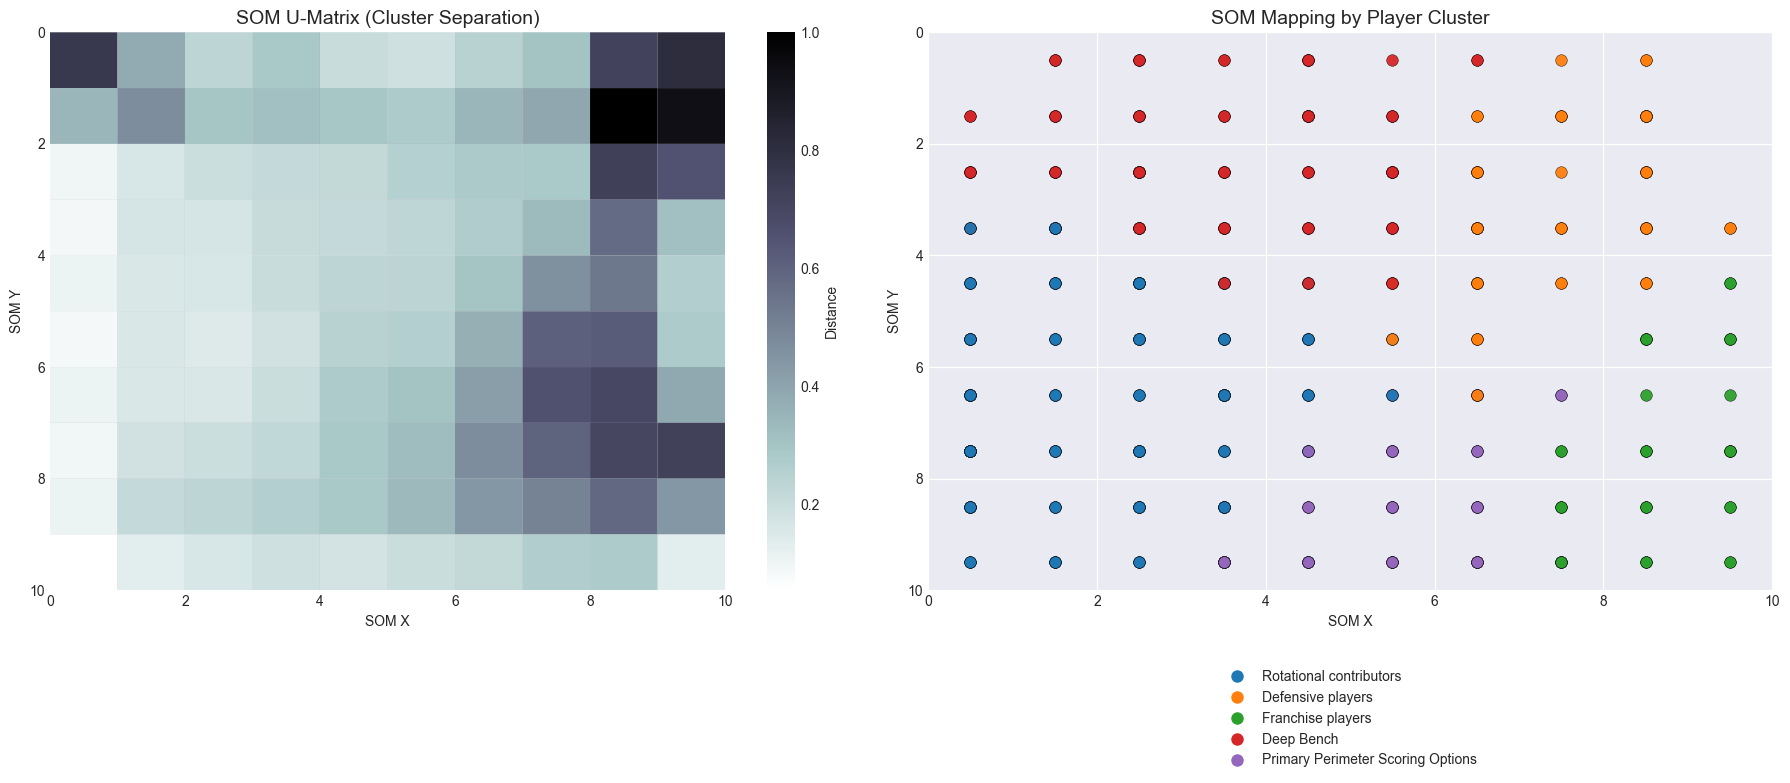
\includegraphics[width=0.7\linewidth]{media/2b.png}
    \caption{SOM U-Matrix showing cluster separation.}
\end{figure}

{\bf Cluster Descriptions:}
\begin{itemize}
    \item \textcolor{blue}{Blue}: Rotational contributors
    \item \textcolor{orange}{Orange}: Defensive players
    \item \textcolor{green}{Green}: Franchise players
    \item \textcolor{red}{Red}: Deep Bench
    \item \textcolor{purple}{Purple}: Primary Perimeter Scoring Options
\end{itemize}

\subsection{Autoencoders + t-SNE}

\begin{table}[h!]
\centering
\caption{Cluster Statistical Summary (mean values per player group)}
\label{tab:cluster_stats}
\begin{tabular}{lcccccc}
\toprule
\textbf{Cluster} & \textbf{PTS} & \textbf{AST\%} & \textbf{STL\%} & \textbf{BLK\%} & \textbf{ORB\%} & \textbf{DRB\%} \\
\midrule
0: Bench role players & 6.98 & 12.19 & 1.52 & 1.47 & 4.00 & 12.83 \\
1: Defensive players & 6.19 & 10.43 & 1.43 & 2.24 & 6.81 & 16.60 \\
2: Secondary playmakers & 13.08 & 16.68 & 1.57 & 1.31 & 3.30 & 12.97 \\
3: Players with limited minutes & 4.93 & 10.13 & 1.44 & 1.92 & 6.65 & 15.37 \\
4: Primary scoring starters & 20.04 & 20.76 & 1.42 & 2.12 & 6.13 & 18.30 \\
\bottomrule
\end{tabular}
\end{table}

This section uses the t-SNE approach which helps us focus on local similarity, preserving players who are close in feature space and it is also useful for visualizing distinct roles clearly. For our interpretation we will make use of the cluster statistical summary and the K-Means clustering.

By using the table of averages above is how we were able to properly describe the clusters:

{\bf Cluster 0:} Bench role players with a moderate average of assists as well as defensive rebounds. Meaning, the players in this cluster are good on defense and they can set up the plays, but lack in scoring stats.

{\bf Cluster 1:} Defensive players. These players tend to be quite tall compared to the others which facilitates in ball possession, and this is backed up by the offensive/defensive rebound averages, however even though they can get a moderate average of assists, their scoring ability is a weakness.

{\bf Cluster 2:} Secondary playmakers also called the 6th man. These players are in charge of setting up the plays, while also being able to score themselves and participate on the defence. They are players who ensure good ball movement on the court, and we see this by looking at the points, average of assists and defensive rebound. 

{\bf Cluster 3:} Players with limited minutes. In the basketball roster the role and talent of a player speaks volumes, and often we get players who are not able to perform at the high level or given opportunities in a team full of talents. Most of these players are quite good on defence and assists, but lack heavily on the scoring sheet.

{\bf Cluster 4:} Starters. These players are all-rounders when it comes to playmaking, scoring and defensive abilities and they compose the 5 main players of the roster.

\begin{figure}[h]
    \centering
    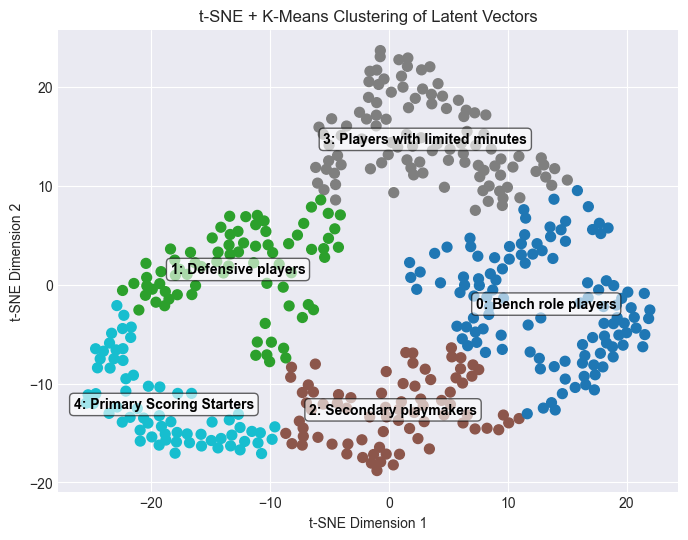
\includegraphics[width=0.7\linewidth]{media/2c.png}
    \caption{t-SNE + K-Means Clustering.}
\end{figure}

\end{document}
